\documentclass[oneside]{book}
\setlength\parindent{24pt}
\usepackage{indentfirst}
\usepackage{lmodern}
\usepackage{color}
\usepackage{listings}
\usepackage{graphicx}
\lstset{ %
language=C++,                % choose the language of the code
basicstyle=\footnotesize,       % the size of the fonts that are used for the code
numbers=left,                   % where to put the line-numbers
numberstyle=\footnotesize,      % the size of the fonts that are used for the line-numbers
stepnumber=1,                   % the step between two line-numbers. If it is 1 each line will be numbered
numbersep=5pt,                  % how far the line-numbers are from the code
backgroundcolor=\color{white},  % choose the background color. You must add \usepackage{color}
showspaces=false,               % show spaces adding particular underscores
showstringspaces=false,         % underline spaces within strings
showtabs=false,                 % show tabs within strings adding particular underscores
frame=single,           % adds a frame around the code
tabsize=2,          % sets default tabsize to 2 spaces
captionpos=b,           % sets the caption-position to bottom
breaklines=true,        % sets automatic line breaking
breakatwhitespace=false,    % sets if automatic breaks should only happen at whitespace
escapeinside={\%*}{*)}          % if you want to add a comment within your code
}
\begin{document}
\title{Unofficial Guide to Interning at Wikia}
\author{Tiffany Perumpail}
\date{August 2015}
\maketitle
\tableofcontents
\chapter{What is this?}
When you join a new team, you have to tackle a huge repository of existing code and a ton of new tools. On top of that, the team will likely have established guidelines for how new code should be written, protocols for the process of committing new code, and a bunch of other unique development practices.\par
The purpose of this guide is to break down the moving parts of the Wikia Services Team into easy-to-understand components. Between IDE's and Mocking Frameworks and Scrum, there will likely be concepts that you are familiar with, as well as concepts that you've never heard of.\par
This guide is meant to be a living document. As time passes, especially in the tech world, tools change. Feel free to update this document as it becomes outdated and new developments occur.
\chapter{How to get started coding}
\section{IntelliJ}
\subsection{Setting up IntelliJ}
The Services Team uses IntelliJ as their Java IDE. The Pandora repository wiki (github.com/Wikia/pandora/wiki/Getting-Started) includes a step-by-step guide on setting up Java and IntelliJ on your machine.
\subsection{I've never used an IDE. What is this and why can't I just use a text editor?}
If used properly, an IDE can save you a ton of time. 
How, you ask?
\begin{itemize}
	\item \textbf{Code Navigation:} \texttt{Command + click} on a function or variable
	\item \textbf{Code Completion:} IntelliJ auto-completes classes and method names as you code. It also expands acronyms (i.e. NPE for "NullPointerException" or "No Page Error."
	\item \textbf{Code Generation:} \texttt{Ctrl + return} can generate getters and setters or implement methods from an interface.
	\item \textbf{Code Coloring:} IntelliJ includes the standard keyword, string, and variable coloring. It also colors member variables, local variables, and parameters.
	\item \textbf{Refactoring:} IntelliJ is extremely effective for mistake-free renaming, even replacing setters, getters, and string usages,
	\item \textbf{Dependency improrting:} When relying on a third party library that you have the source for, you can navigate to the code easily for reference.
	\item \textbf{Debugging:} A 
\end{itemize}
\section{Gradle}
Gradle is an extensive build tool and dependency manager for programming projects. Gradle also provides build-by-convention support for many types of projects including Java, Android and Scala.
\subsection{What is a build script?}
Your build scripts are how you tell Gradle how to build your application. The application itself can be represented by many Gradle projects. A Gradle project does not represent your application as a whole, but instead can represent many different things. It could represent a library jar file you want to build for your project, it could be a distribution zip file, or it could just represent something you want done with the app, such as deploying it to a server.\par
One benefit of having multiple projects in a single application is that it simple to have separate dependencies or to build tasks for the different application parts.\par
How does Gradle know what counts as a project in your application? It will create a project for each 'build.gradle' file in your application. On the previous example, both the Mobile and Wear directories in a Wear application would have a 'build.gradle' file letting Gradle know that it is a separate project. For each project in your build, Gradle will create a Project object. This object allows you to access Gradle features such as adding tasks, properties and dependencies. Properties are defined in the 'build.gradle' file, typically in an extra block.
\section{Jrebel}
JRebel instantly reloads changes to Java code and saves developers time. It works as a java agent on top of the JVM. It looks for changes in the folder with your compiled classes. If you compile a class, JRebel notices the change and compares the differences between class definitions. Then at the bytecode level it adds/removes/replaces fields/method bodies/etc. without restarting the JVM.\par
The JRebel Activation Code can be provided by Nelson.
\section{Project Lombok}
Lombok is a tool that generates code for you, but not in the way that your IDE generates it. Your IDE generates getters and setters, or equals and more, and then puts the code in your uncompiled class file. Lombok generates the same thing, but does it in the class file; all you need to do is add some annotations like \texttt{@Setter}, \texttt{@Getter}, \texttt{@Builder}, \texttt{@Data}, etc. to your code and Lombok generates the setters, getters and so on for you. At the same time, you can override whatever is generated by just writing the method yourself instead.\par
Below is an example of using lombok to generate getters and setters using the \texttt{@Data} annotation. \texttt{@Builder} creates a builder for this class, while \texttt{@AllArgsConstructor} and \texttt{@NoArgsConstructor} create constructors:\par
\begin{figure}[h!]
\centering
	\includegraphics[scale=0.5]{lombok.png}
\end{figure}
\chapter{What is Git and why do we use it?}
\section{What is Git?}
Git is a version control system, or VCS. Specifically, it is a distributed VCS.
\section{Why version control?}
Nobody likes to lose their work. Maybe you're the type of person who constantly pounds the "Save" button on your documents or stores all his files in the cloud. VCS address that paranoia. It helps you track changes to your code.\par
Version Control Systems provide a documented history. As you make changes to your code, you will eventually reach a good stopping point. To save the current status of your project, you still mark the files you changed and "commit" your changes to the VCS. The VCS will store exactly how your code looked at that moment. If you make more changes later, but look back and decide that your new changes are bad, you can always restore your code to a previous commit.\par
Version Control Systems also allow teams to work together, all using the same files. If you've ever tried to edit a document with multiple people (without using Google Drive), you've likely run into issues where somebody edits an older version and is stuck adding their changes to the current version. Or worse, they send out their version and overwrite all the new changes. Using git, there is one remote repository that everyone on our team can work on, make locally make changes to, commit their changes to, and pull changes from when the repository is updated.
\section{What is a repository?}
A repository, or "repo", is a directory where your projects can live. Wikia/pandora is a remote repository on Github. You will also have a local repository on your computer. 
\section{What is my local repository?}
Your local repository is a copy of all the files in the remote repository on your own machine. Your local repository
\subsection{I want to start coding! How do I set up my local repository?}
\noindent Download git for OS X (https://git-scm.com/downloads)\par
\noindent Create your working copy of Wikia/pandora:\par
1. Navigate to the folder on your machine where you want to store your local repo.\par
2. Use the terminal for the following command: git clone https://github.com/Wikia/pandora.git \par
\noindent You have a working copy of the entire pandora repository!
\subsection{I got my first ticket! What do I do?}
\noindent Make a branch with your ticket name.\par
This command creates a local copy of all the files in master.\par
\texttt{>>> git branch SERVICES-000} \par
\noindent This command allows you to start working on your branch.\par
\texttt{>>> git checkout SERVICES-000} \par
\noindent Now, you can start making your changes on this branch!
\chapter{What is TunnelBlick?}
Tunnelblick is a free, open source graphic user interface for OpenVPN on OS X. It provides easy control of OpenVPN client and/or server connections.
\section{What is a VPN?}
A VPN or Virtual Private Network is a network connection that enables you to create a secure connection over the public Internet to private networks at a remote location. With a VPN, all network traffic (data, voice, and video) goes through a secure virtual tunnel between the host device (client) and the VPN provider's servers, and is encrypted. VPN technology uses a combination of features such as encryption, tunneling protocols, data encapsulation, and certified connections to provide you with a secure connection to private networks and to protect your identity.\par
VPN connections technically give you all the benefits of a Local Area Network (LAN), which is similar to that found in many offices but without requiring a hard-wired connection.\par
VPNs are often set up to give individual employees secure remote access to their company networks, hence the name "virtual private network". By connecting to the company's network, an individual employee can access all the company's resources and services as if the employee were inside the company.
\begin{figure}[h!]
\centering
	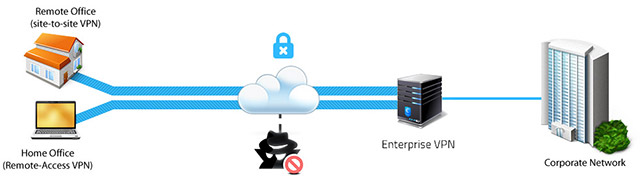
\includegraphics[scale=0.3]{VPN.png}
	\caption{VPN connecting to a Corporate Network}
\end{figure}
\section{What is OpenVPN?}
OpenVPN is an open-source software application that implements virtual private network (VPN) techniques for creating secure point-to-point or site-to-site connections in routed or bridged configurations and remote access facilities. It uses a custom security protocol that utilizes SSL/TLS for key exchange.
\chapter{How do I debug?}
The first three things I double-check when my code isn't working in the office are:
\begin{itemize}
	\item Am I connected to VPN?
	\item Have I configured my environment variables and argument?
	\item Have I synced Gradle?
\end{itemize}
If none of these checks reveal the problem, then we'll have to delve into using the IntelliJ Debugger.
\section{IDE Debugging}
\subsection{Why use an IDE debugger?}
You may be thinking, why do I need a debugger? I can already look at trace messages in my code. What more do I need!\par
Here are some benefits of using an IDE debugger:
\begin{itemize}
	\item Add \textbf{breakpoints} to temporarily suspend execution of your program at a certain point (No more print-statement debugging!)
	\item Be able to  \textbf{watch variables} and see when they change
	\item Conditional breakpoints; stop the application only in exceptional circumstances to allow you to analyse the stack and variables.
	\item View the call stack at any point in time, giving you a context for your current stack frame.
	\item Change variable values while the program is running
	\item Be able to skip or repeat sections of code, to see how the code will perform. This allows you to test out theoretical changes before making them.
	\item Alert you when certain exceptions are thrown, even if they are handled by the application.
\end{itemize}
\subsection{What are breakpoints?}
A breakpoint is a signal that tells the debugger to temporarily suspend execution of your program at a certain point. When execution is suspended at a breakpoint, your program is said to be in break mode. Entering break mode does not terminate or end the execution of your program. Execution can be resumed at any time.\par
You can think of break mode as being like a timeout. All the elements remain, functions, variables, and objects remain in memory, for example, but their movements and activities are suspended. During break mode, you can examine their positions and states to look for violations or bugs. You can make adjustments to the program while in break mode. You can change the value of a variable, for example. You can move the execution point, which changes the statement that will be executed next when execution resumes.\par
Breakpoints are a powerful tool for pinpointing where a problem is occurring in your code. Rather than stepping through your code line-by-line or instruction-by-instruction, you can allow your program to run until it hits a breakpoint, then start to debug. This speeds up the debugging process enormously. Without this ability, it would be virtually impossible to debug a large program.\newpage
\subsection{How do I do all this in IntelliJ?}
Below is an example screenshot of using the debugger in IntelliJ. By clicking on the gray section to the left of your code, you can add break points, which are represented by red circles (see below). In order to run your code in debug mode, click the green "bug" icon next to the standard run icon. Then, once you hit a breakpoint, you can navigate to the variable tabs on the lower portion of your window to view the current state of the variables. \newline
\newline\begin{flushright}

\end{flushright}
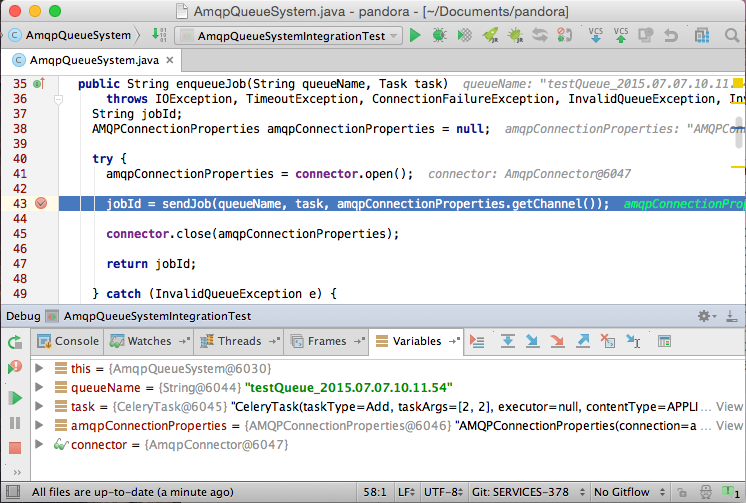
\includegraphics[scale=0.5]{intellijdebugger.png}
\chapter{How do I test my code?}
When you are developing your code, you can always manually test your code. However, manual tests are the worst kind of tests because there is no log of those tests and they are difficult to reproduce. Therefore, the team creates thorough unit and end-to-end tests for all new code.
\section{What are unit tests?}
A unit test is a test written by the programmer to verify that a relatively small piece of code is doing what it is intended to do. It should have \textbf{no dependencies} on code outside of the section being tested. They are narrow in scope, they should be easy to write and execute, and their effectiveness depends on what the programmer considers to be useful. The tests are intended for the use of the programmer, they are not directly useful to anybody else, though, if they do their job, testers and users downstream should benefit from seeing fewer bugs.\par
Part of being a unit test is the implication that things outside the code under test are mocked or stubbed out. Unit tests shouldn't have dependencies on outside systems. They test internal consistency as opposed to proving that they play nicely with some outside system.
\section{What are End-To-End / Integration tests?}
An end-to-end / integration test is done to demonstrate that different pieces of the system work together. Integration tests cover whole applications, and they require much more effort to put together. They usually require resources like database instances and hardware to be allocated for them. The integration tests do a more convincing job of demonstrating the system works (especially to non-programmers) than a set of unit tests can, at least to the extent the integration test environment resembles production.\par
These tests are referred to as end2end tests in the Helios repo and integration tests in the Pandora repo, but they are the same thing.
\section{What is cobertura?}
Cobertura is a free Java tool that calculates the percentage of code accessed by tests. It can be used to identify which parts of your Java program are lacking test coverage. You can run cobertura through gradle, by clicking on the command shown below.\par
\begin{figure}[h!]
\centering
	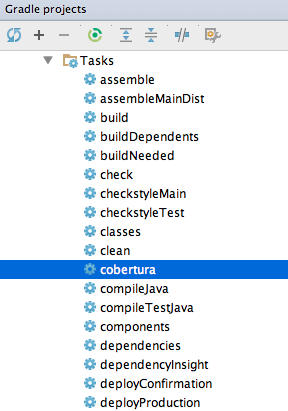
\includegraphics[scale=0.4]{cobertura.png}
\end{figure}
After running this command, you can access the report generated in a reports/cobertura folder. An example report is provided below:
\begin{figure}[h!]
\centering
	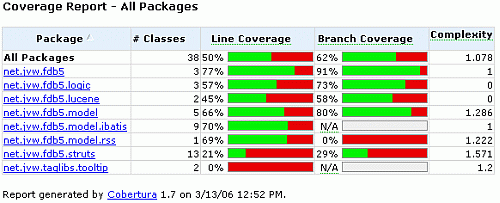
\includegraphics[scale=0.6]{coberturareport.png}
\end{figure}
\subsection{What is line coverage?}
Line coverage measures how many statements you took (a statement is usually a line of code, not including comments, conditionals, etc). The line coverage report represents \textbf{the percent of lines executed by the test run}.
\subsection{What is branch coverage?}
Branch coverages checks if you took the true and false branch for each conditional (if, while, for). You'll have twice as many branches as conditionals. The branch coverage report represents \textbf{the percent of branches executed by the test run}.
\subsection{Why should I care about the difference between line coverage and branch coverage?}
Consider the following example: \\
\begin{lstlisting}
public int getNameLength(boolean isCoolWikiaIntern) {
    User user = null;
    if (isCoolWikiaIntern) {
        user = new Connie(); 
    }
    return user.getName().length(); 
}
\end{lstlisting}
If you call this method with \texttt{isCoolWikiaIntern} set to true, you get 100\% line coverage. That sounds great, until you realize that there will be a \texttt{NullPointerException} if you call with \texttt{isCoolUser} set to false. However, you have 50\% branch coverage in the first case, so you can see there is something missing in your testing (and often, in your code).
\section{Mocking}
\subsection{Mockito}
\chapter{How do I contribute to meetings?}
Whenever you are the newest joining member of a group, the rest of the members will have accumulated knowledge about the project that you are not privy to. Add being an intern fresh out of college on top of that, and team meetings can seem pretty intimidating.\par
Instead of dwelling on these fears, let's talk about how to mitigate them. This chapter will specifically focus on Scrum-style meetings, but the sentiments can be applied to joining any pre-existing team.
\section{Using their Accumulated Knowledge}
No one in the meeting knows everything about all the moving parts. Usually, the team members have specialized knowledge on different aspects of the project. Use that to your advantage! If you don't know something, ASK. Odds are you aren't the only one who doesn't know all the ins and outs of the topic at hand.\par
Additionally, explaining a project component in detail can be helpful to the developer, too. Being able to clearly and concisely explain what you are doing and why you are doing it is a major part of development. 
\section{Accumulating your own knowledge}
\subsection{Backlog Grooming}
During backlog grooming, the team comes together to look over the tickets in the backlog. They add new stories and epics, extract stories from existing epics, and estimate effort for existing stories. Basically, this is your chance to get up to date on everything you missed before you joined the team! Pay close attention during these meetings to understand what every story consists of and ask questions about anything you don't understand.
\subsection{Sprint Planning}
Every iteration begins with the sprint planning meeting. At this meeting, the Product Owner and the team negotiate which stories a team will tackle that sprint. During this meeting, you have a chance to fully understand all of the stories that the team will be working on this sprint and be up to date with what everyone on the team is doing. \par
When you estimate the amount of effort for each story, you will gain a better understanding of all that moving parts that the story involves. 

Take advantage of this meeting! It will help you stay up-to-date on all the upcoming stories and contribute meaningfully in future meetings.
\chapter{Mistakes I've made}
Git, I deleted a file without knowing it. (Ended up spending half and hour debugging the issue before going to Nelson.)
Wrote interfaces that were so specific they didn't serve a purpose.
Not everyday will be your best day, don't be too hard on yourself.
\end{document}